% 第一章 项目概述
\section{项目概述}

\subsection{项目简介}

\textbf{智舆}是一款面向城市治理的AI智慧舆情态势监测感知与决策推演系统,旨在通过人工智能技术赋能传统舆情监测,构建集\textbf{数据采集、智能分析、3D可视化展示、走向预测、决策模拟}于一体的综合性平台。

系统核心价值在于:\textbf{让城市管理者"看得见"舆情态势、"听得懂"民意诉求、"想得清"发展走向、"做得好"科学决策}。

本项目采用\textbf{讯飞星火4.0大模型}作为核心AI分析引擎,结合\textbf{高德地图3D可视化}、\textbf{多Agent决策推演}、\textbf{城市模型矩阵}、\textbf{语音交互播报}等创新技术,实现从舆情监测到辅助决策的全流程智能化。系统支持\textbf{全国-省份-地级-县级}四级区域穿透分析,可根据文字、图片、视频等多模态舆情内容AI生成现场3D模型,并通过决策模拟功能帮助用户预判不同应对策略的效果。创新性地构建\textbf{城市模型矩阵},基于LoRA微调技术为不同城市/省份训练专属适配器,实现本地化舆情精准分析。

项目首期聚焦\textbf{信阳市}场景落地,逐步扩展至河南省乃至全国城市,为政府、企业、个人提供差异化的舆情智慧服务。

\subsection{项目背景}

\subsubsection{政策背景}

\textbf{国家层面}高度重视智慧城市与数字政府建设。2025年10月,国家发改委等五部门联合印发《深化智慧城市发展推进全域数字化转型行动计划》,明确提出到2027年底建成50个以上全域数字化转型城市。《国务院关于加强数字政府建设的指导意见》确立了到2025年政府数字化履职能力框架基本形成的目标。

\textbf{河南省层面},《河南省深化智慧城市发展推进城市全域数字化转型实施方案(2025-2027年)》提出打造3-5个国内一流的综合型城市全域数字化转型标杆。《河南省支持人工智能产业生态发展若干政策措施》提供真金白银支持:对通过国家生成式AI模型备案的企业给予100万元资金支持,设立30亿元人工智能产业基金。

\textbf{信阳市层面},《信阳市数字政府建设实施方案(2023-2025年)》确立了数字化转型的总体框架,12345热线系统已升级为舆情监测重要平台。

\begin{figure}[H]
\centering
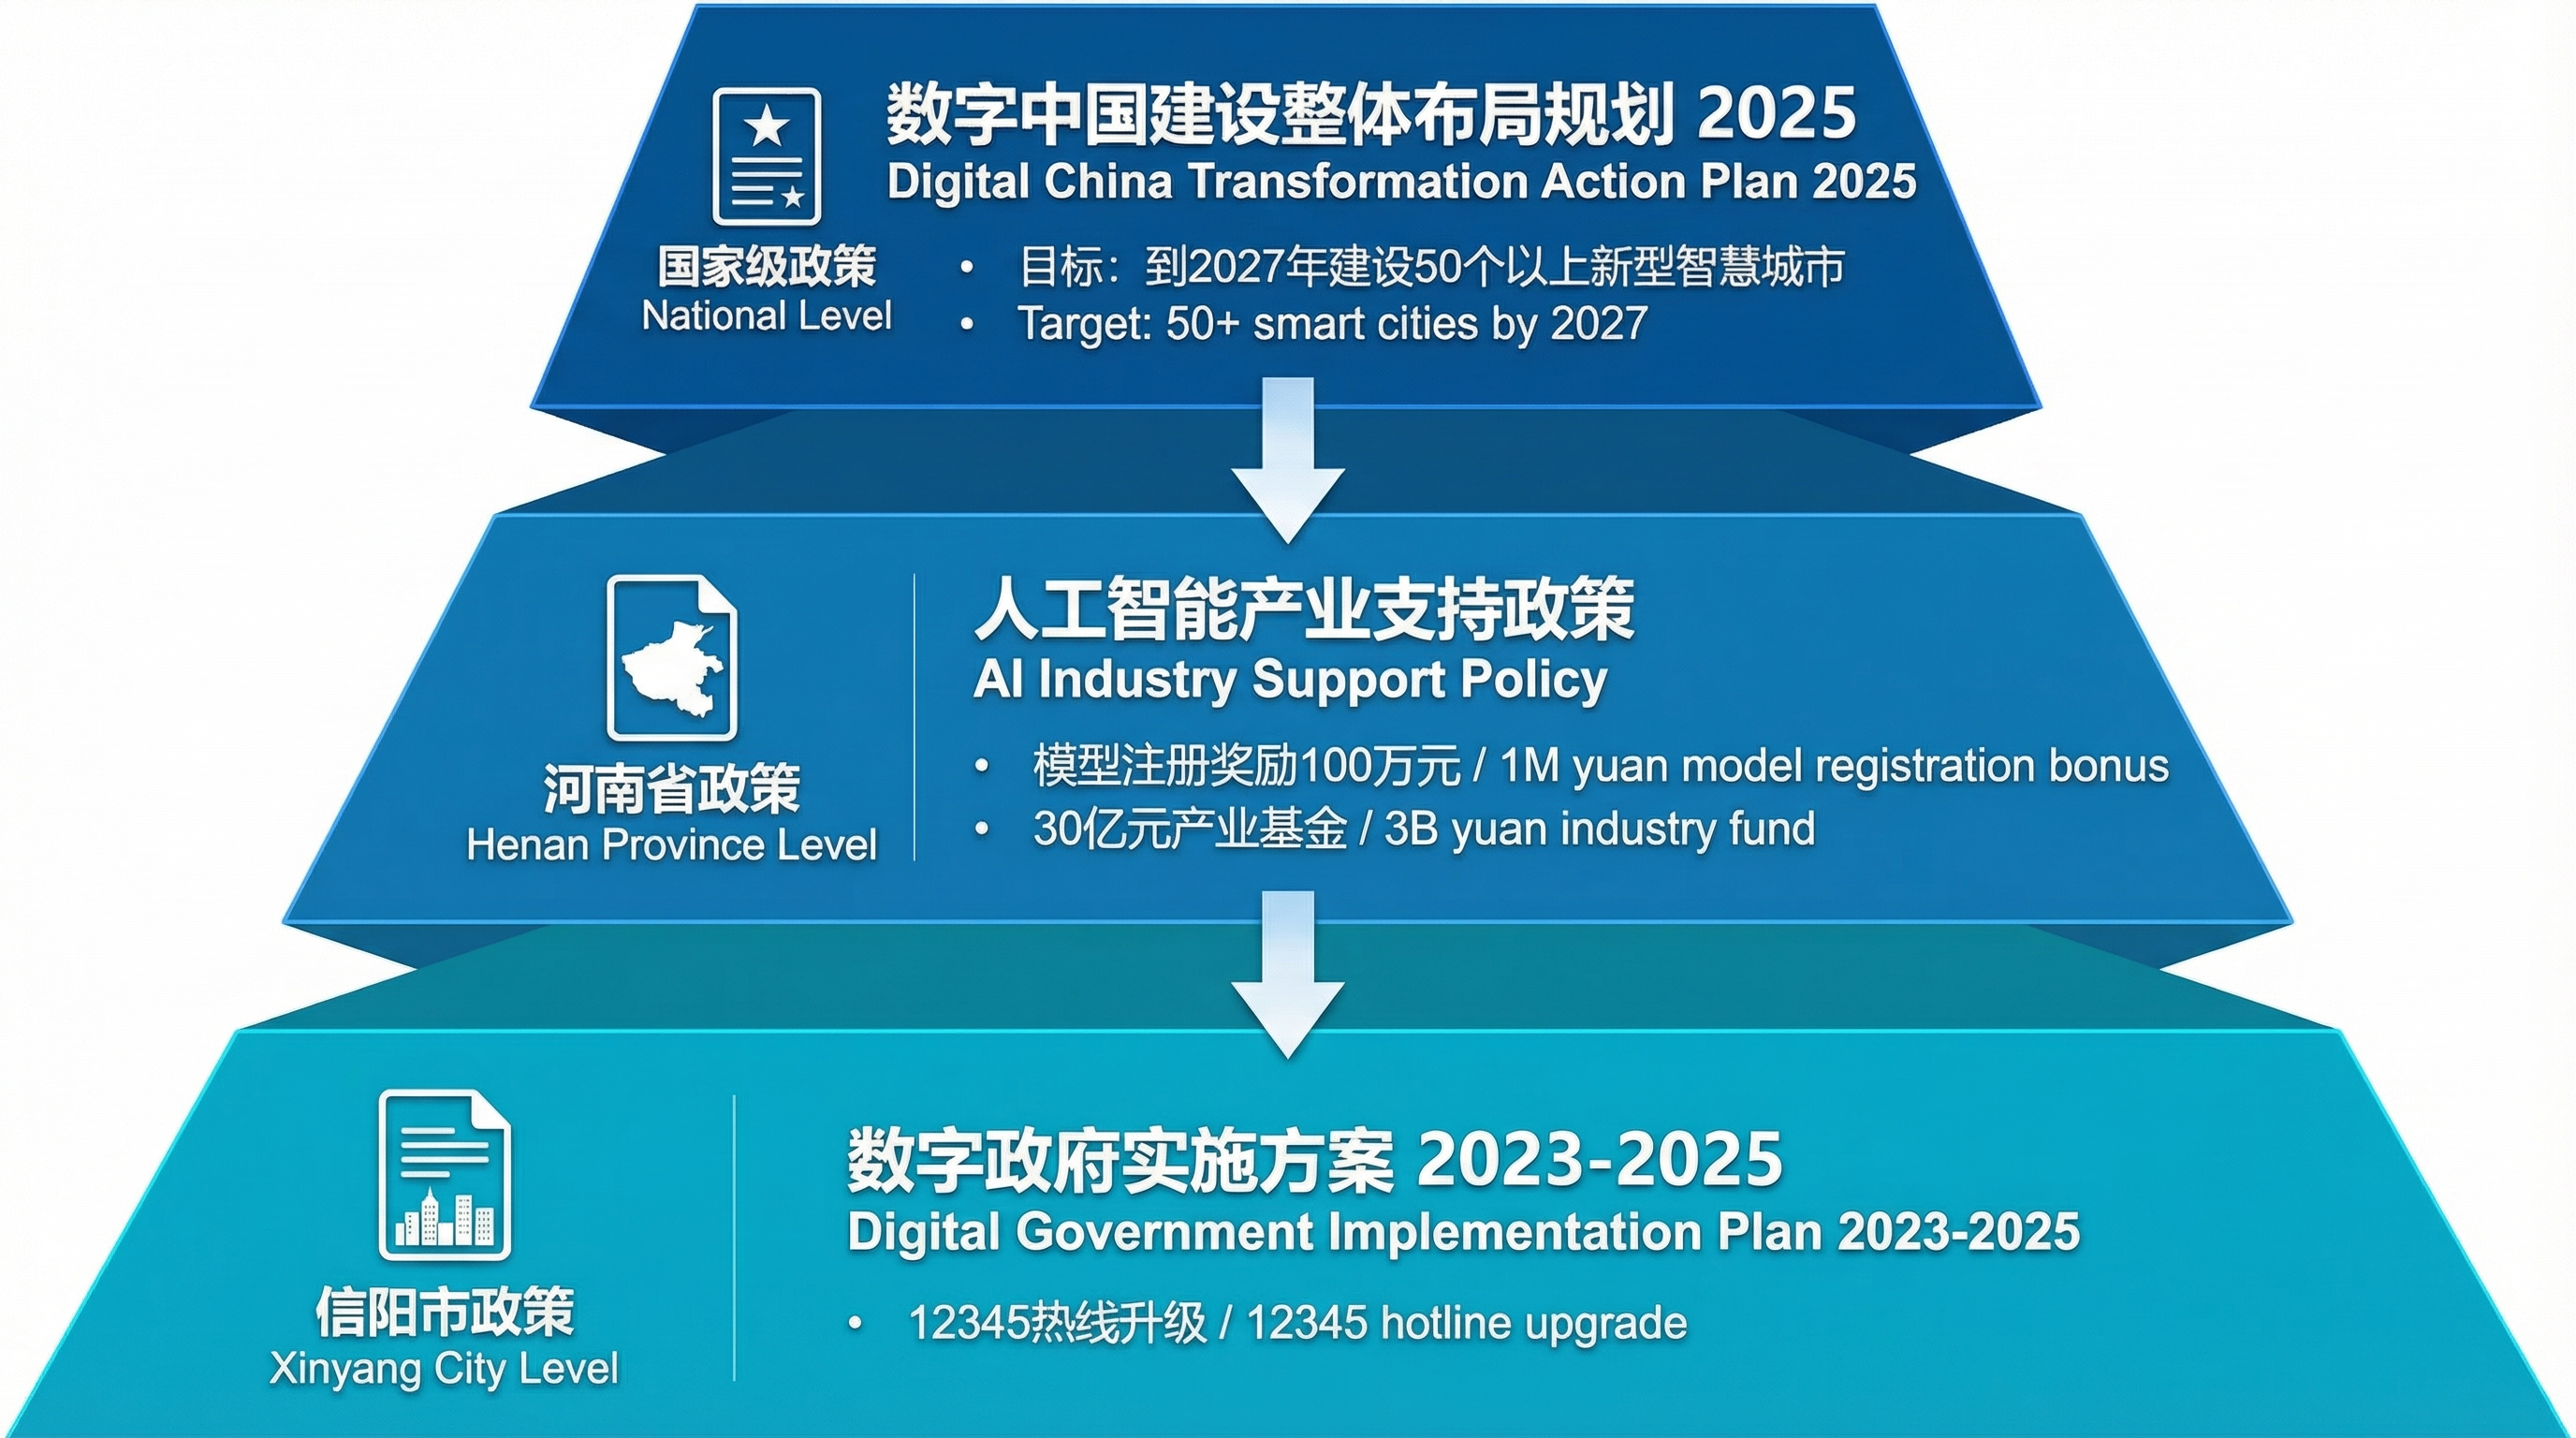
\includegraphics[width=0.85\textwidth]{../picture/fig01_policy_system.png}
\caption{国家-省-市三级政策支持体系图}
\end{figure}

\subsubsection{行业背景}

\textbf{舆情监测市场高速增长}。根据行业调研数据,2024年全球舆情监测系统市场规模约23.15亿美元,预计2031年将达40.50亿美元,年复合增长率8.1\%\textsuperscript{[5]}。中国市场增速领跑全球,2025年预计突破72.4亿元人民币,增速高达26.4\%\textsuperscript{[6]}。

\textbf{行业痛点亟待解决}。当前舆情监测行业存在五大核心痛点:一是\textbf{数据覆盖不全},主流产品聚焦头部平台,对中小网站、短视频、图片等多模态内容的覆盖不足,漏检率高达15-30\%;二是\textbf{智能化程度低},传统系统依赖关键词匹配和人工审核,日均需投入3-5名分析师进行舆情研判,效率低下且成本高昂;三是\textbf{可视化单一},绝大多数产品仍采用传统2D图表和列表展示,难以直观呈现舆情的时空分布与演化态势;四是\textbf{决策支持弱},现有系统侧重于监测和分析环节,缺乏走向预测和决策模拟能力,用户"只知道发生了什么"却"不知道该怎么办";五是\textbf{下沉市场空白},主流产品年费动辄数万至数十万元,地级市、县区及中小企业难以承担,形成显著的市场空白。

\begin{figure}[H]
\centering
\includegraphics[width=0.85\textwidth]{../picture/fig02_market_trend.png}
\caption{中国舆情监测市场规模增长趋势图(2020-2030)}
\end{figure}

\subsubsection{技术背景}

\textbf{大模型技术突破}为智能舆情分析提供了可能。2025年,GPT-5、讯飞星火4.0等主流大模型在情感分析基准测试上的准确率已达94.7\%,远超传统方法的75-85\%\textsuperscript{[8]}。

\textbf{3D可视化技术成熟}。WebGL、Three.js、高德地图JS API 2.0等技术已广泛应用于三维城市可视化场景。

\textbf{AI 3D生成技术兴起}。Tripo AI、TripoSR等工具可在10秒内将文字/图片转换为3D模型。

\subsubsection{地域特色}

\textbf{信阳市}作为河南省地级市,具有独特的区位优势和发展需求,是本项目理想的首批落地场景。信阳地处鄂豫皖三省交界,是著名的革命老区,红色文化资源丰富,舆情场景具有鲜明地域特色。作为中国十大名茶"信阳毛尖"的原产地,茶产业相关的品牌舆情、消费维权、产地保护等议题关注度持续较高。信阳市常住人口超过600万,民生诉求呈现多元化特征,涵盖交通出行、教育医疗、环境保护、消费维权等多个领域。目前信阳市已建成12345市民服务热线平台,初步具备数字政务基础,但智能化分析能力仍有较大提升空间,亟需引入AI技术实现舆情监测的智能化升级。

\subsection{项目优势}

\subsubsection{技术优势}

\begin{table}[H]
\centering
\caption{技术优势总览}
\begin{tabular}{L{3cm}L{10cm}}
\toprule
\textbf{优势维度} & \textbf{具体内容} \\
\midrule
大模型驱动 & 深度集成讯飞星火4.0 Ultra,128K上下文,情感识别准确率超90\% \\
多Agent协作 & 基于LangGraph构建分析-预测-决策-模拟四Agent协作体系 \\
3D可视化 & 高德地图3D + Three.js,支持全国-省-市-县四级穿透 \\
AI场景还原 & Tripo AI生成舆情现场3D模型,实现"看见新闻现场" \\
语音交互 & 讯飞TTS/ASR实现语音播报预警与语音指令控制 \\
轻量化部署 & 云原生架构,支持SaaS订阅,降低使用门槛 \\
\bottomrule
\end{tabular}
\end{table}

\subsubsection{团队优势}

本项目团队具备完成系统开发所需的综合能力。在\textbf{专业构成}方面,团队成员涵盖计算机科学、大数据技术、人工智能等相关专业背景,形成了前端开发、后端架构、AI算法、产品设计等多角色协作的团队结构。在\textbf{技术储备}方面,团队成员具备Web全栈开发、数据可视化、机器学习模型调用等项目实践经历,熟悉Vue3、Python、FastAPI、讯飞星火API等核心技术栈,前端原型已开发完成并验证了技术路线的可行性。在\textbf{本地资源}方面,团队立足信阳学院,对信阳市政务需求和本地舆情特征有切身了解,便于开展需求调研、用户访谈和试点推广,具备"接地气"的产品设计优势。

\subsubsection{差异化优势}

\begin{table}[H]
\centering
\caption{差异化优势对比}
\begin{tabular}{L{2.5cm}L{5cm}L{5.5cm}}
\toprule
\textbf{对比维度} & \textbf{主流产品} & \textbf{智舆系统} \\
\midrule
目标市场 & 省级/大型企业 & 地级市/县域/中小企业 \\
价格定位 & 3-100万元/年 & 万元级/免费增值模式 \\
可视化方式 & 2D图表为主 & 3D地图沉浸式体验 \\
决策支持 & 监测+分析 & 监测+分析+预测+模拟 \\
部署方式 & 私有化为主 & SaaS+轻量化私有化 \\
AI生成能力 & 无 & 舆情场景3D模型生成 \\
\bottomrule
\end{tabular}
\end{table}
